
\begin{figure*}[bt]
\begin{center}
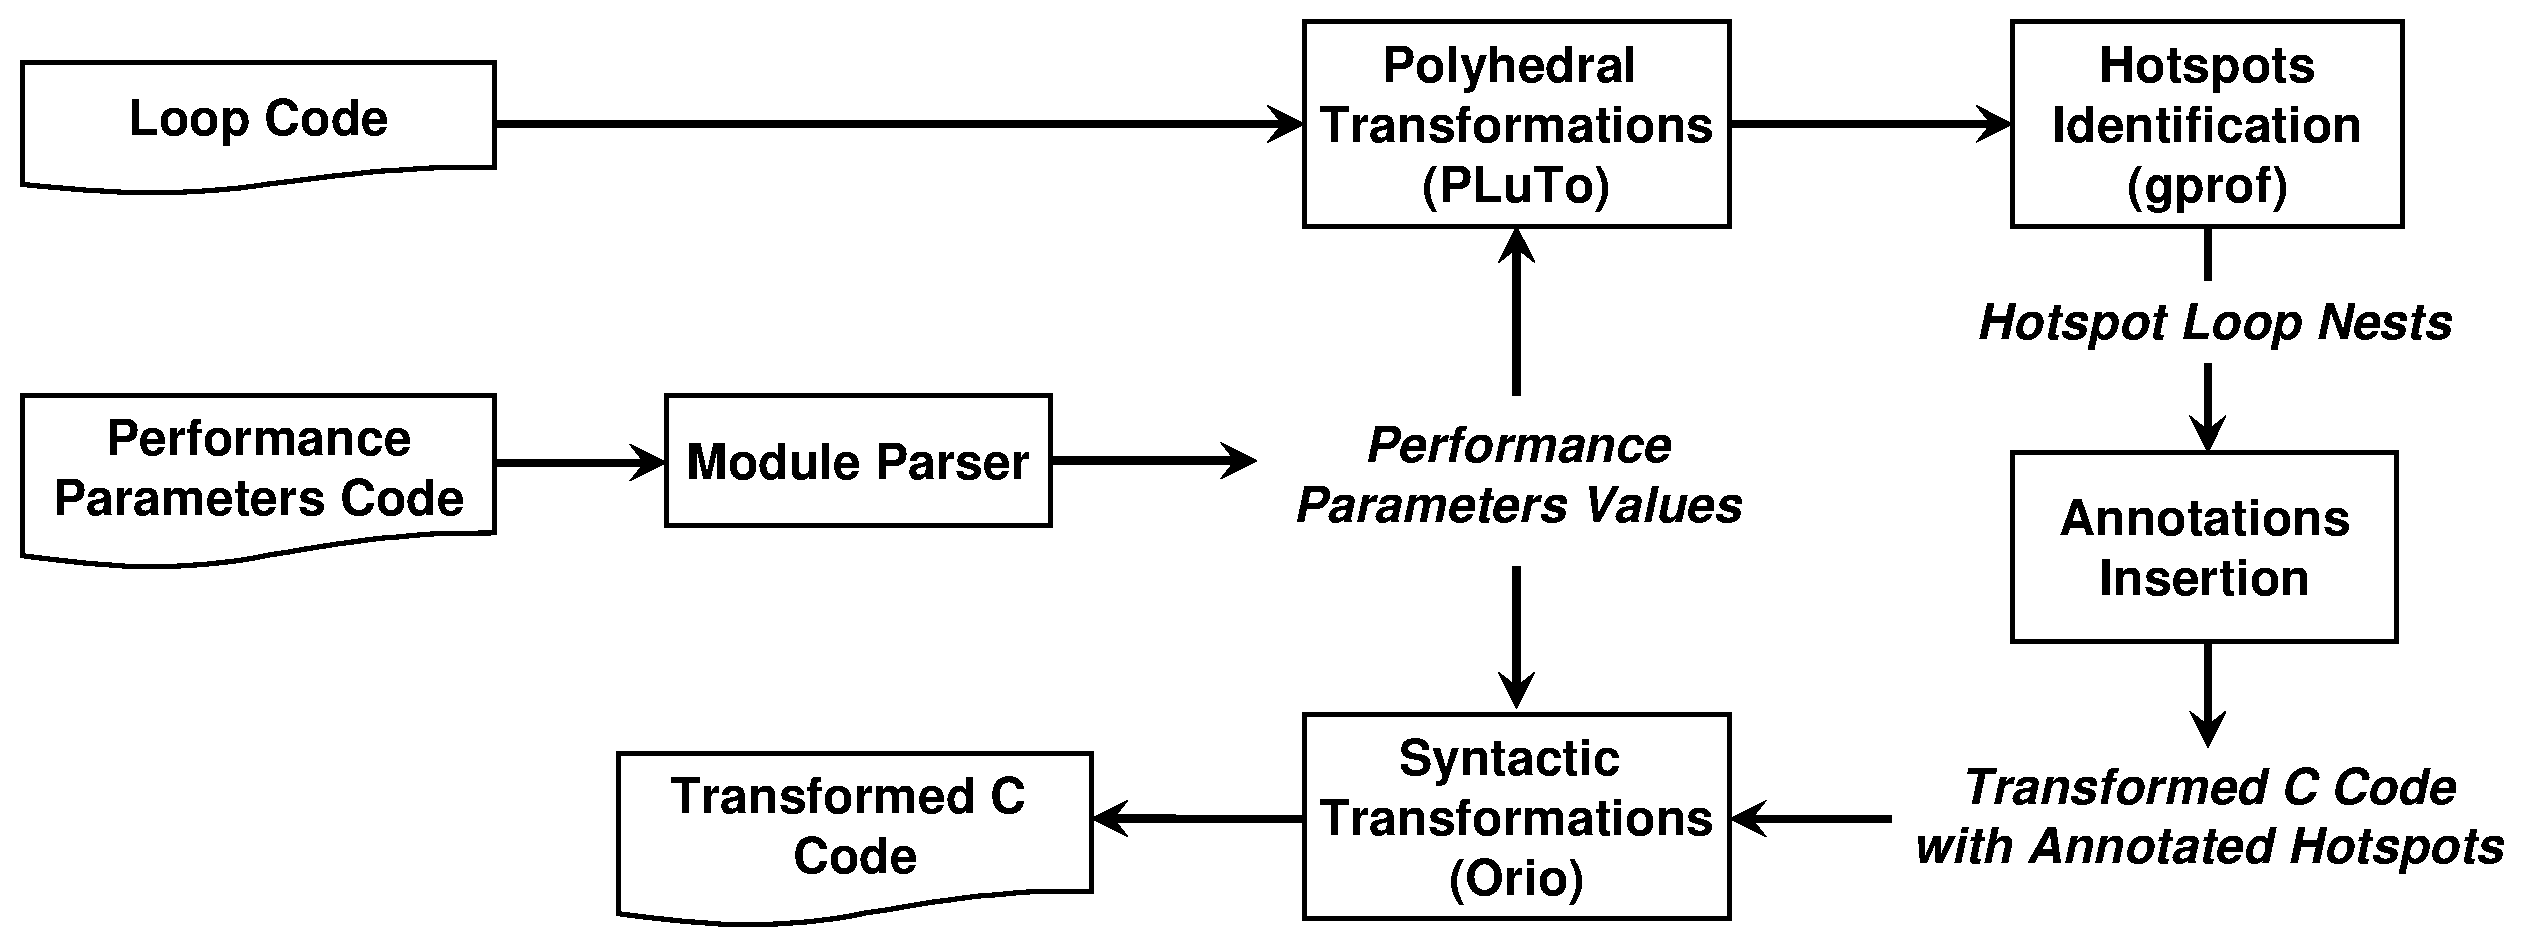
\includegraphics[width=0.6\textwidth]{figures/pluto-orio.eps}    
\end{center}   
\caption{Integration of Pluto into Orio's code transformation module.}
\label{fig:pluto-orio}
\end{figure*}  

\section{Pluto-Orio Integration}
\label{sec:integration}

A number of source-to-source transformation tools for performance
optimization exist. Using these tools to achieve (near) optimal performance
on different architectures, however, is still a nontrivial task that requires
significant architectural and compiler expertise. By combining code
transformation tools with an empirical tuning system, such as Orio, we can
reduce the amount of manual effort and automatically determine the
transformations that result in the best performance. We show in this section
how Orio has been extended with an external transformation program, called
Pluto~\cite{uday08pldi}. This integration also demonstrates the easy
extensibility of Orio and the ability to leverage other source transformation
approaches.

Pluto is a source-to-source automatic transformation tool aimed at optimizing
a sequence of nested loops for data locality and coarse-grained parallelism
simultaneously. Pluto employs a polyhedral model of arbitrary loop nests,
where the dynamic instance (iteration) of each statement is viewed as an
integer point in a well-defined space called the statement's polyhedron. This
statement representation and a precise characterization of data dependences
enable Pluto to construct mathematically correct complex loop
transformations. Pluto's polyhedral-based transformations result in improved
cache locality and loops parallelized for multicore architecture.

Figure~\ref{fig:pluto-orio} outlines the overall structure of the
Pluto-Orio integrated system, which is implemented as a new
optimization module in Orio. Initially, the transformation process
takes two kinds of input: the loop code to be optimized and the
optimization parameters code. The loop code is embedded in the
annotation body block, while the performance parameters code is
written in the module body block. A parser implemented inside
the new module parses the performance parameters code to extract their
values. The extracted values of the performance parameters include
tile sizes, unroll factors, loop order (permutation), as well as
several boolean values for triggering OpenMP parallelization, scalar
replacement, and auto-vectorization. Using these parameter values,
Pluto then performs polyhedral transformations (e.g., two-level tiling
and OpenMP parallelization) on the input loop code. The resulting
generated code is subsequently passed to the widely-available
profiling tool gprof~\cite{gprof} for hotspot detection. The
statistical information produced by gprof provides accurate locations
(line numbers) of the loop nests where the Pluto-generated code spends
most of its execution time. The identified hotspot loop nests are then
decorated with Orio's performance annotations for complementary
syntactic transformations (e.g., loop permutation, loop
unroll/jamming, scalar replacement, and explicit
auto-vectorization). Finally, Orio optimizes the annotated hotspots as
described in Section~\ref{sec:implm}.

Pluto also performs syntactic loop unroll/jam in a post-processing
pass. The target loops, however, are limited only to innermost loops with a
maximum depth of two (i.e., 1-D unrolling and 2-D unroll/jamming). So we
choose to use the loop unroll/jam transformation already available in
Orio, which is more flexible because it can be applied to loop nests of
depths larger than two.



At present Orio does not employ any data dependence analysis when performing
syntactic transformations. Therefore, there is no guarantee that the code
generated after syntactic transformations is correct. Because of this, the
tuning process using the integrated Pluto-Orio system is currently
semi-automatic---user involvement is required to decide whether it is safe
to apply a syntactic transformation on an identified hotspot.
%The user only needs
%to check the transformation legalities once, since the hotspots
%consistently have similar basic loop structure for different
%Pluto-generated code versions. Once all illegal syntactic
%transformations are known by the user, they must be switched off so
%that the tuning process can proceed fully automatic with no more human
%interventions.



